% !TEX root = summary-ipcv.tex
\section{Punktbildoperation}


\subsubsection{Bildverarbeitung}
\begin{itemize}
	\itemsep0pt
	\item \textbf{Computergrafik:} Erzeugung von realistischen Bildern aus der Beschreibung von Objekten. Beispielsweise werden realistische Bilder erzeugt und dann als Trainingsdaten für Machine Learning Applikationen verwendet.
	\item \textbf{Bildverarbeitung:} Erkennung von Objekten oder Szenen aus Bildern.
\end{itemize}

\subsubsection{Bildverarbeitung auf verschiedenen Stufen}
\begin{center}
	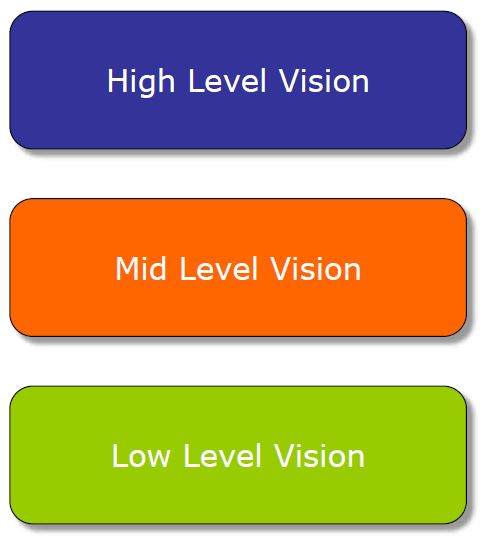
\includegraphics[height=3cm,keepaspectratio]{images/sw01/StufenBildverarbeitung.JPG}
\end{center}

\begin{itemize}
	\itemsep0pt
	\item Computer Vision (High Level Vision): Interpretation des Bildes, Erkennung von Objekten. 
	\item Image Processing (Low Level Vision): Bildverbesserung (Kontrastkorrektur, Rauschunterdrückung), Erkennung von Low Level Features (Kanten, Linien,...)
\end{itemize}


\subsection{Bildverarbeitungs-Methoden}
Bevor Methoden angewendet werden, werden Bilder oft vorverarbeitet. D.h. Informationen verstärken oder Störungen reduziert.
\newline
\newline
Unterscheidung zwischen:
\begin{itemize}
	\itemsep0pt
	\item \textbf{Punktoperatoren:} Operation auf einem Punkt. Nur der Grau- (oder Farb-) wert wird transformiert.
	\item \textbf{Nachbarschaftsoperatoren:} Ergebnis hängt von der Umgebung des Punktes ab. zB. 3x3 Umgebung, Filteroperationen, etc.
\end{itemize}

\paragraph{RGB Übersicht}
R(Rot)G(Grün)B(Blau). Werte gegen 0 werden dunkler, Werte gegen 255 hingegen heller.



\begin{center}
	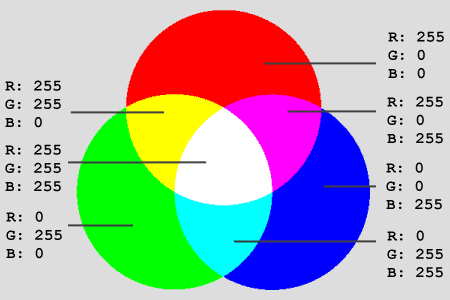
\includegraphics[height=4.5cm,keepaspectratio]{images/sw01/rgb-farbmodell.png}
\end{center}

\noindent\fbox{%
	\parbox{\textwidth}{%
		\textbf{OpenCV} liest Bilder in BGR-Format. Mit image\_rgb = cv2.cvtColor(image, cv2.COLOR\_BGR2RGB) können Bilder in das RGB-Format konvertiert.
	}%
}




\subsection{Punktbildfunktionen}
Veränderung der Intensitätswerte durch eine Funktion. Beispiele: Schwellwert, Helligkeitsveränderung, Kontrast Korrektur, Gamma Korrektur.

\subsubsection{Helligkeitsveränderung}
Im Beispiel wird Helligkeit erhöht, erkennbar durch die Verschiebung der Kurve nach oben. Die Werte im Histogramm verschieben sich somit nach rechts.
\begin{center}
	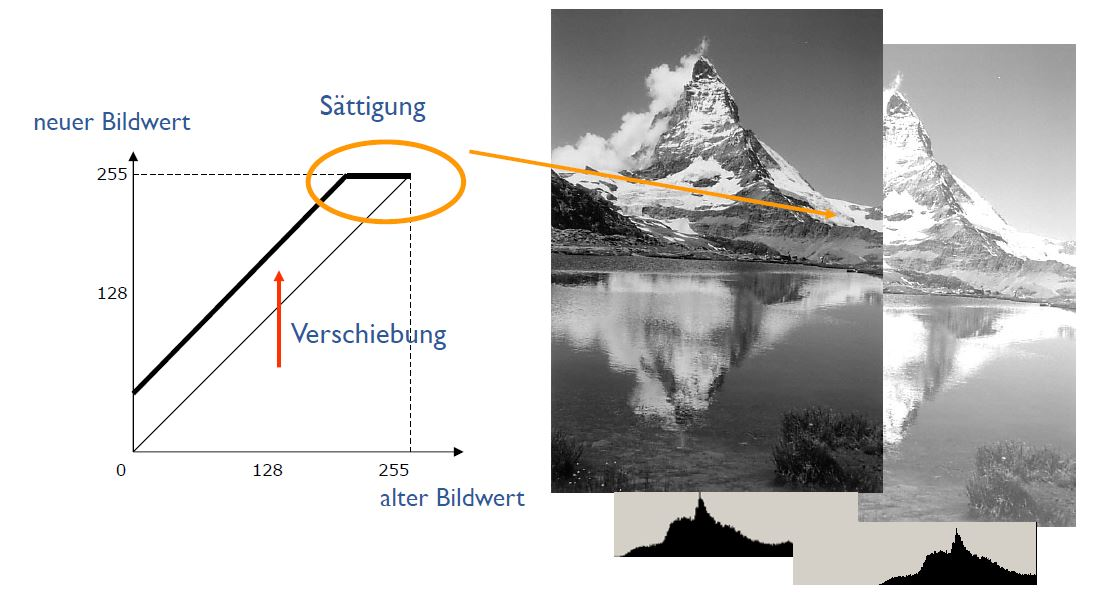
\includegraphics[height=6cm,keepaspectratio]{images/sw01/Helligkeitsveraenderung.JPG}
\end{center}

\noindent\fbox{%
	\parbox{\textwidth}{%
		\textbf{OpenCV:} Methode zum verändern der Helligkeit \newline
		\begin{center}
			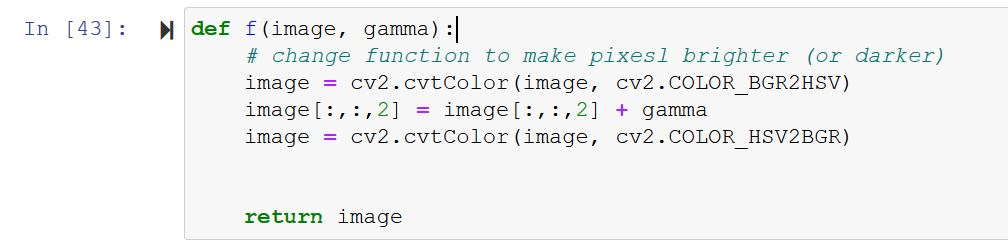
\includegraphics[height=3cm,keepaspectratio]{images/sw01/OpenCVHelligkeit.JPG}
		\end{center}
	}%
}


\subsubsection{Kontrastveränderung}
Wenn die Steigung $>$ 1 ist, dann nimmt die Kontrastveränderung zu. Falls nicht, nimmt sie ab. Optimal ist eine Kurve mit einer S-Form, da so am wenigsten Informationen verloren gehen.
\begin{center}
	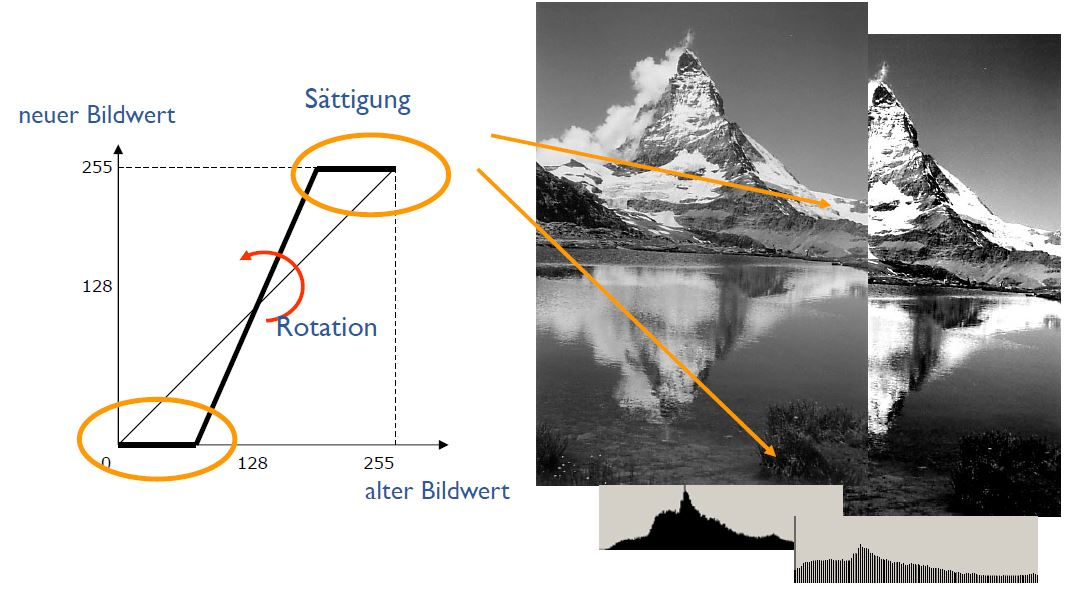
\includegraphics[height=6cm,keepaspectratio]{images/sw01/Kontrastveraenderung.JPG}
\end{center}

\subsubsection{Gamma-Korrektur}
Die vom Menschen empfundene Helligkeit steigt in dunklen Bereichen steiler und in hellen weniger steil an. Die Stevenssche Potenzfunktion ordnet dem menschlichen Auge dabei ein Gamma von ca. 0,3 bis 0,5 zu. Soll das Helligkeitssignal eines Anzeigegerätes, beispielsweise eines Monitors, linear wahrgenommen werden, muss es daher mit dem reziproken des obigen Gammawerts (ca. 3,3 bis 2) vorverzerrt werden, damit sich beide Nichtlinearitäten für den Betrachter am Ende wieder aufheben. Ein typischer Wert für Bildschirme ist etwa ein Gamma von 2,2

\begin{center}
	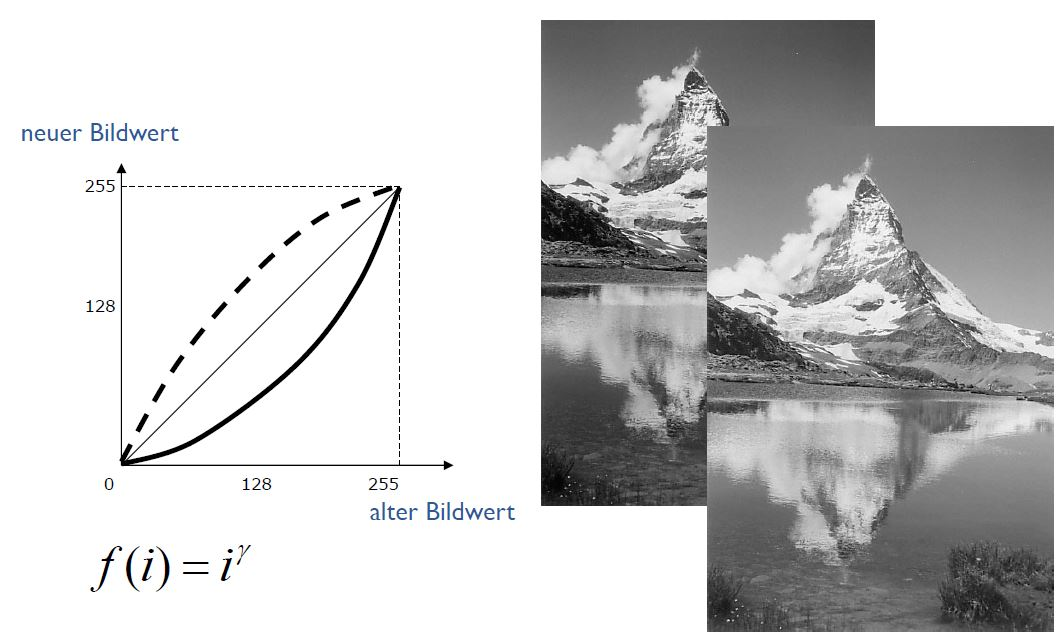
\includegraphics[height=6cm,keepaspectratio]{images/sw01/Gammakorrektur.JPG}
\end{center}

Je nach Grösse des Exponenten $\gamma$(gamma) unterscheidet man 3 Fälle:
\begin{itemize}
	\itemsep0pt
	\item $\gamma$ = 1: die Abbildung ist linear.
	\item $\gamma <$ 1: Die Abbildung ist konkav. Kleine Eingabewerte werden stark gespreizt, grosse gestaucht. (gepunktete Linie)
	\item $\gamma >$ 1: Die Abbildung ist konvex. Kleine Eingabewerte werden gestaucht, grosse gespreizt. (durchgezogene Linie)
\end{itemize}



\subsection{Histogramm}
Farbverteilung des Bildes: Wie häufig kommt welche Farbe/Helligkeit vor. So kommen im ersten Beispiel unten häufig sehr dunkle Werte vor, was auch gut erkennbar im Histogramm ist.

\begin{center}
	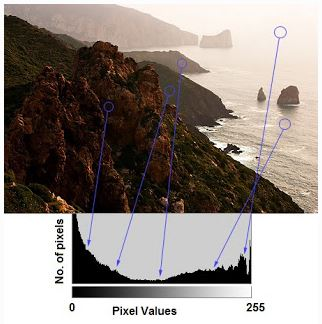
\includegraphics[height=7cm,keepaspectratio]{images/sw01/BspHistogramm.JPG}
\end{center}
\begin{center}
	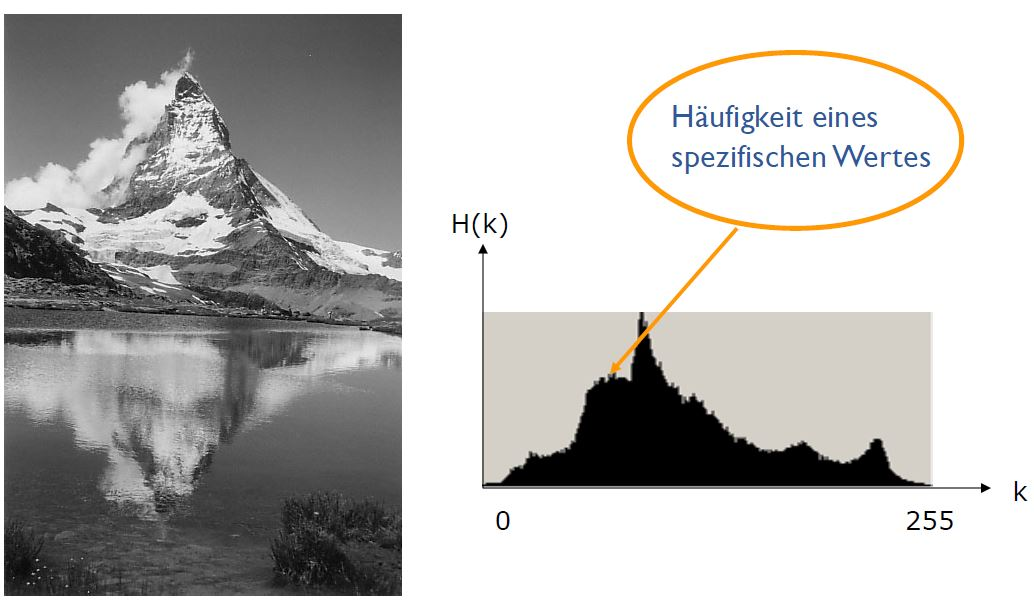
\includegraphics[height=6cm,keepaspectratio]{images/sw01/BspHistogramm2.JPG}
\end{center}

\noindent\fbox{%
	\parbox{\textwidth}{%
		\textbf{OpenCV} cv2.calcHist(images/sw01, channels, mask, histSize, ranges[, hist[, accumulate]])
		\begin{itemize}
			\itemsep0pt
			\item \textbf{1.} images/sw01 : it is the source image of type uint8 or float32. it should be given in square brackets, ie, “[img]”. 
			\item \textbf{2.} channels : it is also given in square brackets. It the index of channel for which we calculate histogram. For example, if input is grayscale image, its value is [0]. For color image, you can pass [0],[1] or [2] to calculate histogram of blue,green or red channel respectively
			\item \textbf{3.} mask : mask image. To find histogram of full image, it is given as “None”. But if you want to find histogram of particular region of image, you have to create a mask image for that and give it as mask. (I will show an example later.)
			\item \textbf{4.} histSize : this represents our BIN count. Need to be given in square brackets. For full scale, we pass [256].
			\item \textbf{5.} ranges : this is our RANGE. Normally, it is [0,256]
		\end{itemize}
		
	}%
}

\subsubsection{Histogrammausgleich}
Ziel eines Histogrammausgleich ist die Transformation der Grauwerte, so dass das Histogramm des neuen Bildes möglich ausgeglichen ist. Die Funktion wird in Bildverarbeitung-Tools oft "Auto Contrast" genannt.
\begin{center}
	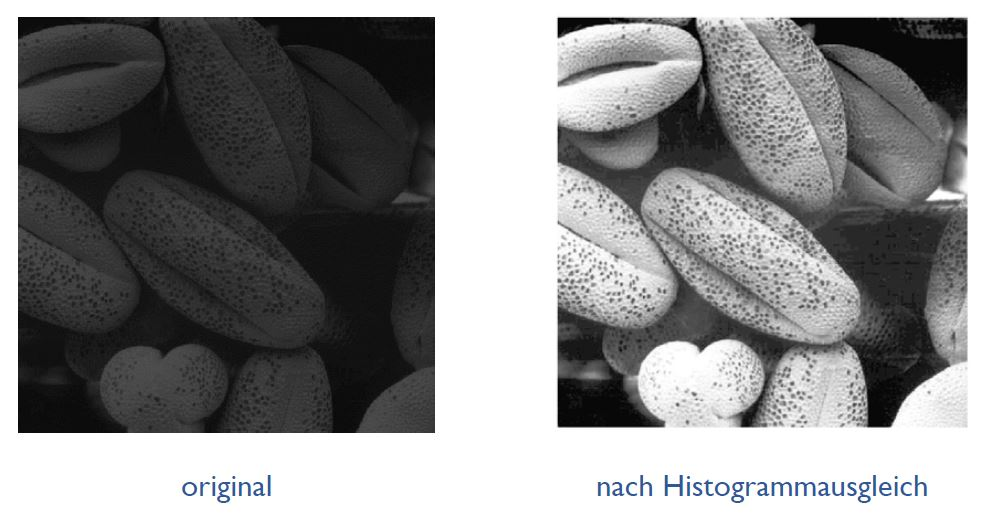
\includegraphics[height=5cm,keepaspectratio]{images/sw01/BspHistogrammausgleich.JPG}
\end{center}

\begin{center}
	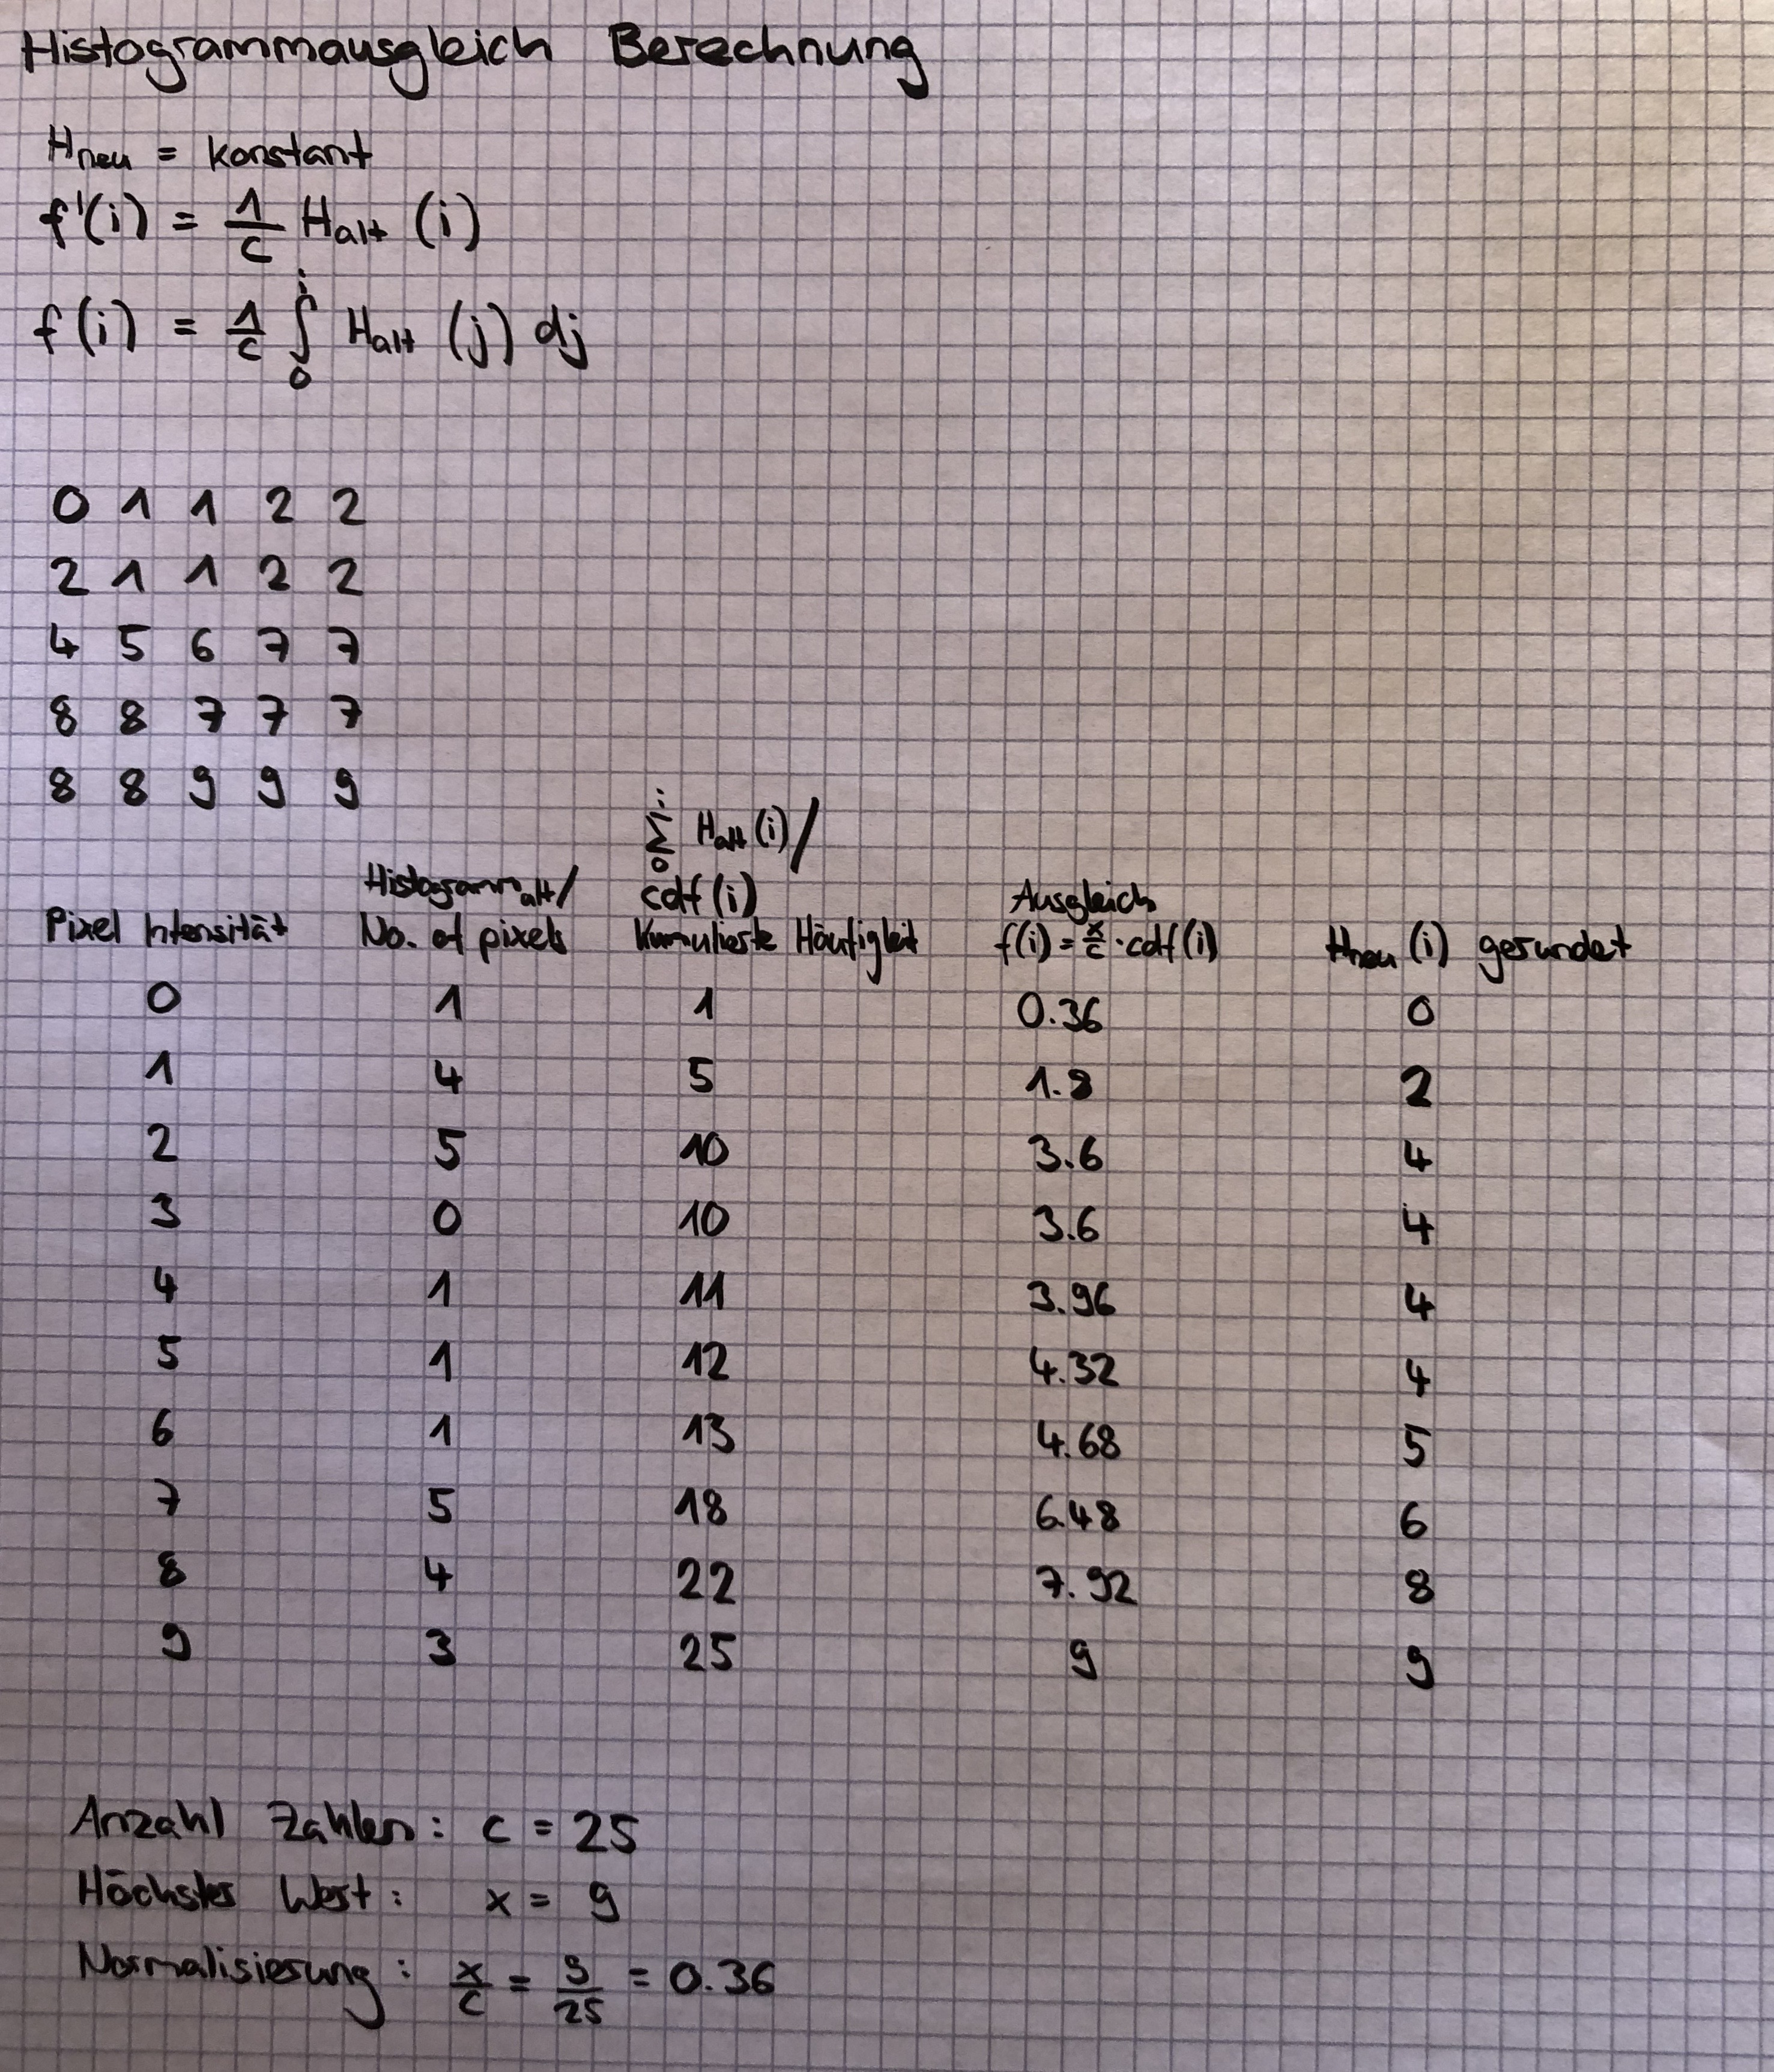
\includegraphics[height=15cm,keepaspectratio]{images/sw01/HistogrammAusgleichBerechnung.JPG}
\end{center}

\subsection{Morphologische Operationen}
\begin{itemize}
	\itemsep0pt
	\item Morphologische Operation werden zur Bearbeitung von Binärbildern verwendet
	\item Binärbilder können zum Beispiel mit dem Setzen eines Schwellwerts (engl. Threshold) erzeugt werden
	\item Die entstehenden Regionen müssen jedoch häufig weiterverarbeitet werden.
	\item Morphologische Operationen benötigen zwei Inputs. Das original Bild und ein Strukturelement (kernel)
	\item Morphologische Operationen können durch Mengenoperationen dargestellt werden. Dabei wird das Bild mit einem Strukturelement verknüpft, dieses ist als Matrix definiert.
\end{itemize}

\subsubsection{Dilate}
Verdickt das Objekt. Wenn mind. 1 Pixel vom Bild unter dem Strukturelement ist. Es vergrössert das Objekt im Vordergrund und entfernt so beispielsweise weisse Löcher. 
\begin{center}
	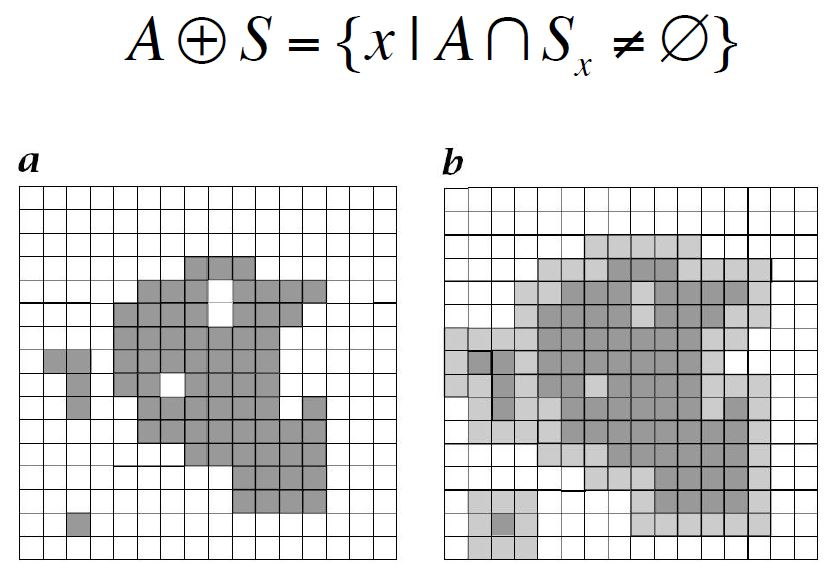
\includegraphics[height=5cm,keepaspectratio]{images/sw01/Dilate.JPG}
\end{center}


\subsubsection{Erode}
Verdünnt das Objekt. Bei Erode muss das ganze Strukturelement über den Pixel des Bildes sein. Ansonsten werden diese entfernt.
\begin{center}
	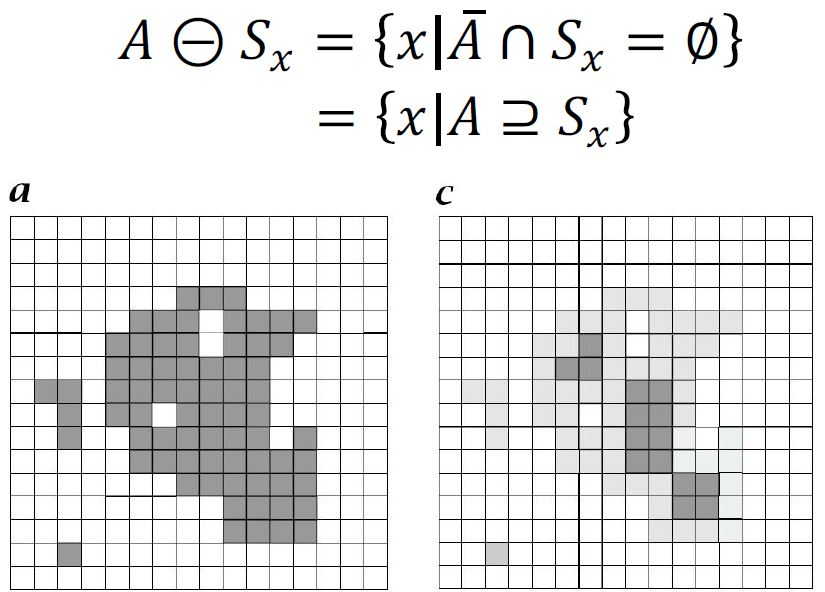
\includegraphics[height=5cm,keepaspectratio]{images/sw01/Erode.JPG}
\end{center}

\subsubsection{Closing/Opening}
\paragraph{Closing} Dilate gefolgt von Erode. Schliesst das Objekt (eliminiert Löcher)

\paragraph{Opening} Erode gefolgt von Dilate. Öffnen (separiert) Objekte. Ist sinnvoll um Störungen aus Bilder zu entfernen


\begin{center}

	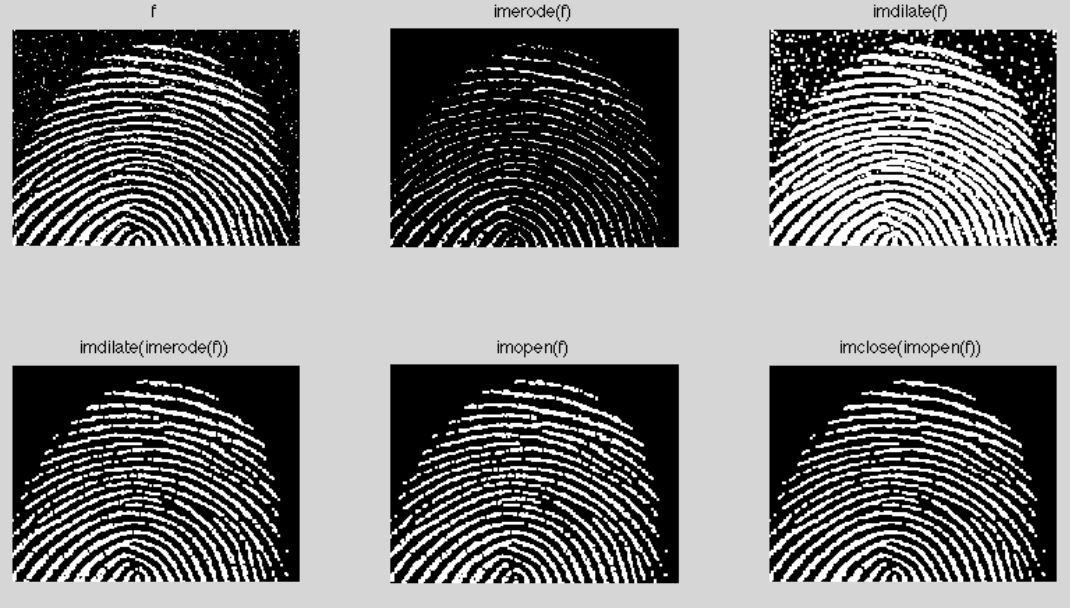
\includegraphics[height=8cm,keepaspectratio]{images/sw01/BspOpenClosing.JPG}
\end{center}

\subsection{Connected Component Labeling}
Auch bekannt als connected component analysis, blob extraction, region labeling, blob discovery oder region extraction. Dabei geht um eine Anwendung aus der Graphentheorie, wo Teilmengen von "connected components" eindeutig markiert (labeled) aufgrund einer gegebenen Heuristik. 

\begin{itemize}
	\itemsep0pt
	\item Wie viele Objekte sind auf einem (binären) Bild zu sehen?
	\item Wie "gross" (Anzahl Pixel) sind Objekte?
	\item Welche Regionen sind zusammenhängend?

\end{itemize}

\begin{center}
	
	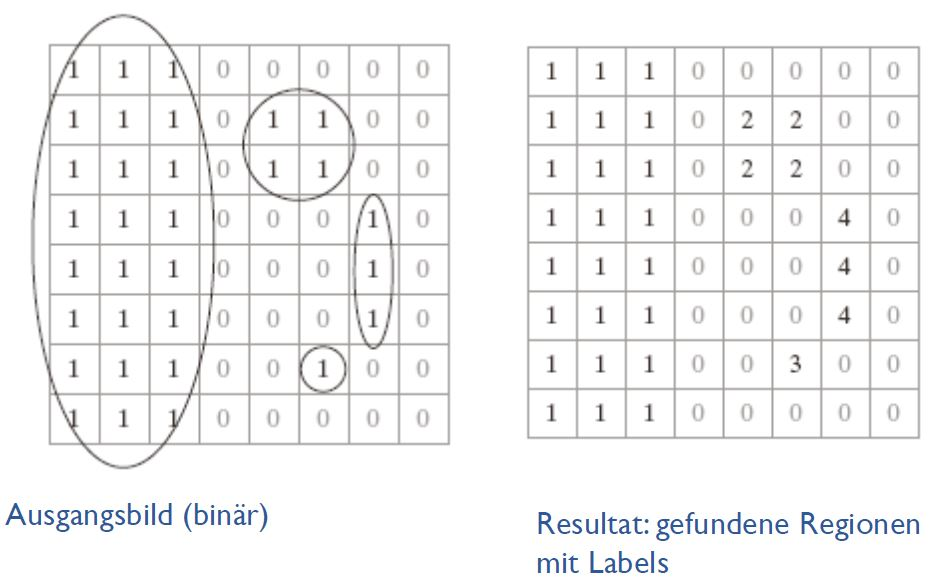
\includegraphics[height=6cm,keepaspectratio]{images/sw01/BspCCL.JPG}
\end{center}

\paragraph{4er/8er Zusammenhang}
\begin{center}
	
	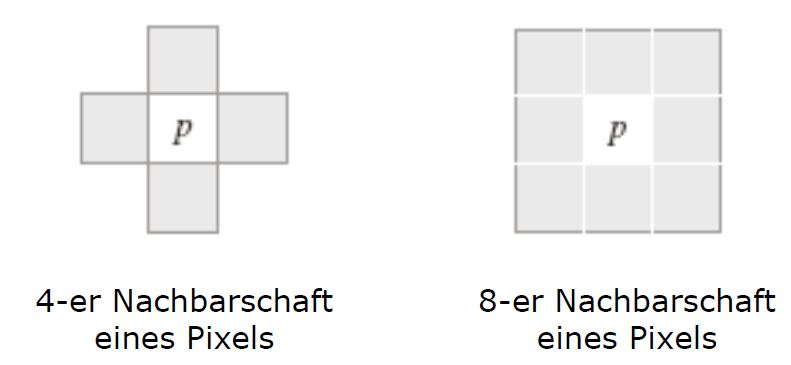
\includegraphics[height=4cm,keepaspectratio]{images/sw01/Nachbarschaften.JPG}
\end{center}


\subsection{Übungen}
\subsubsection{Spiegelung} 
\begin{center}
	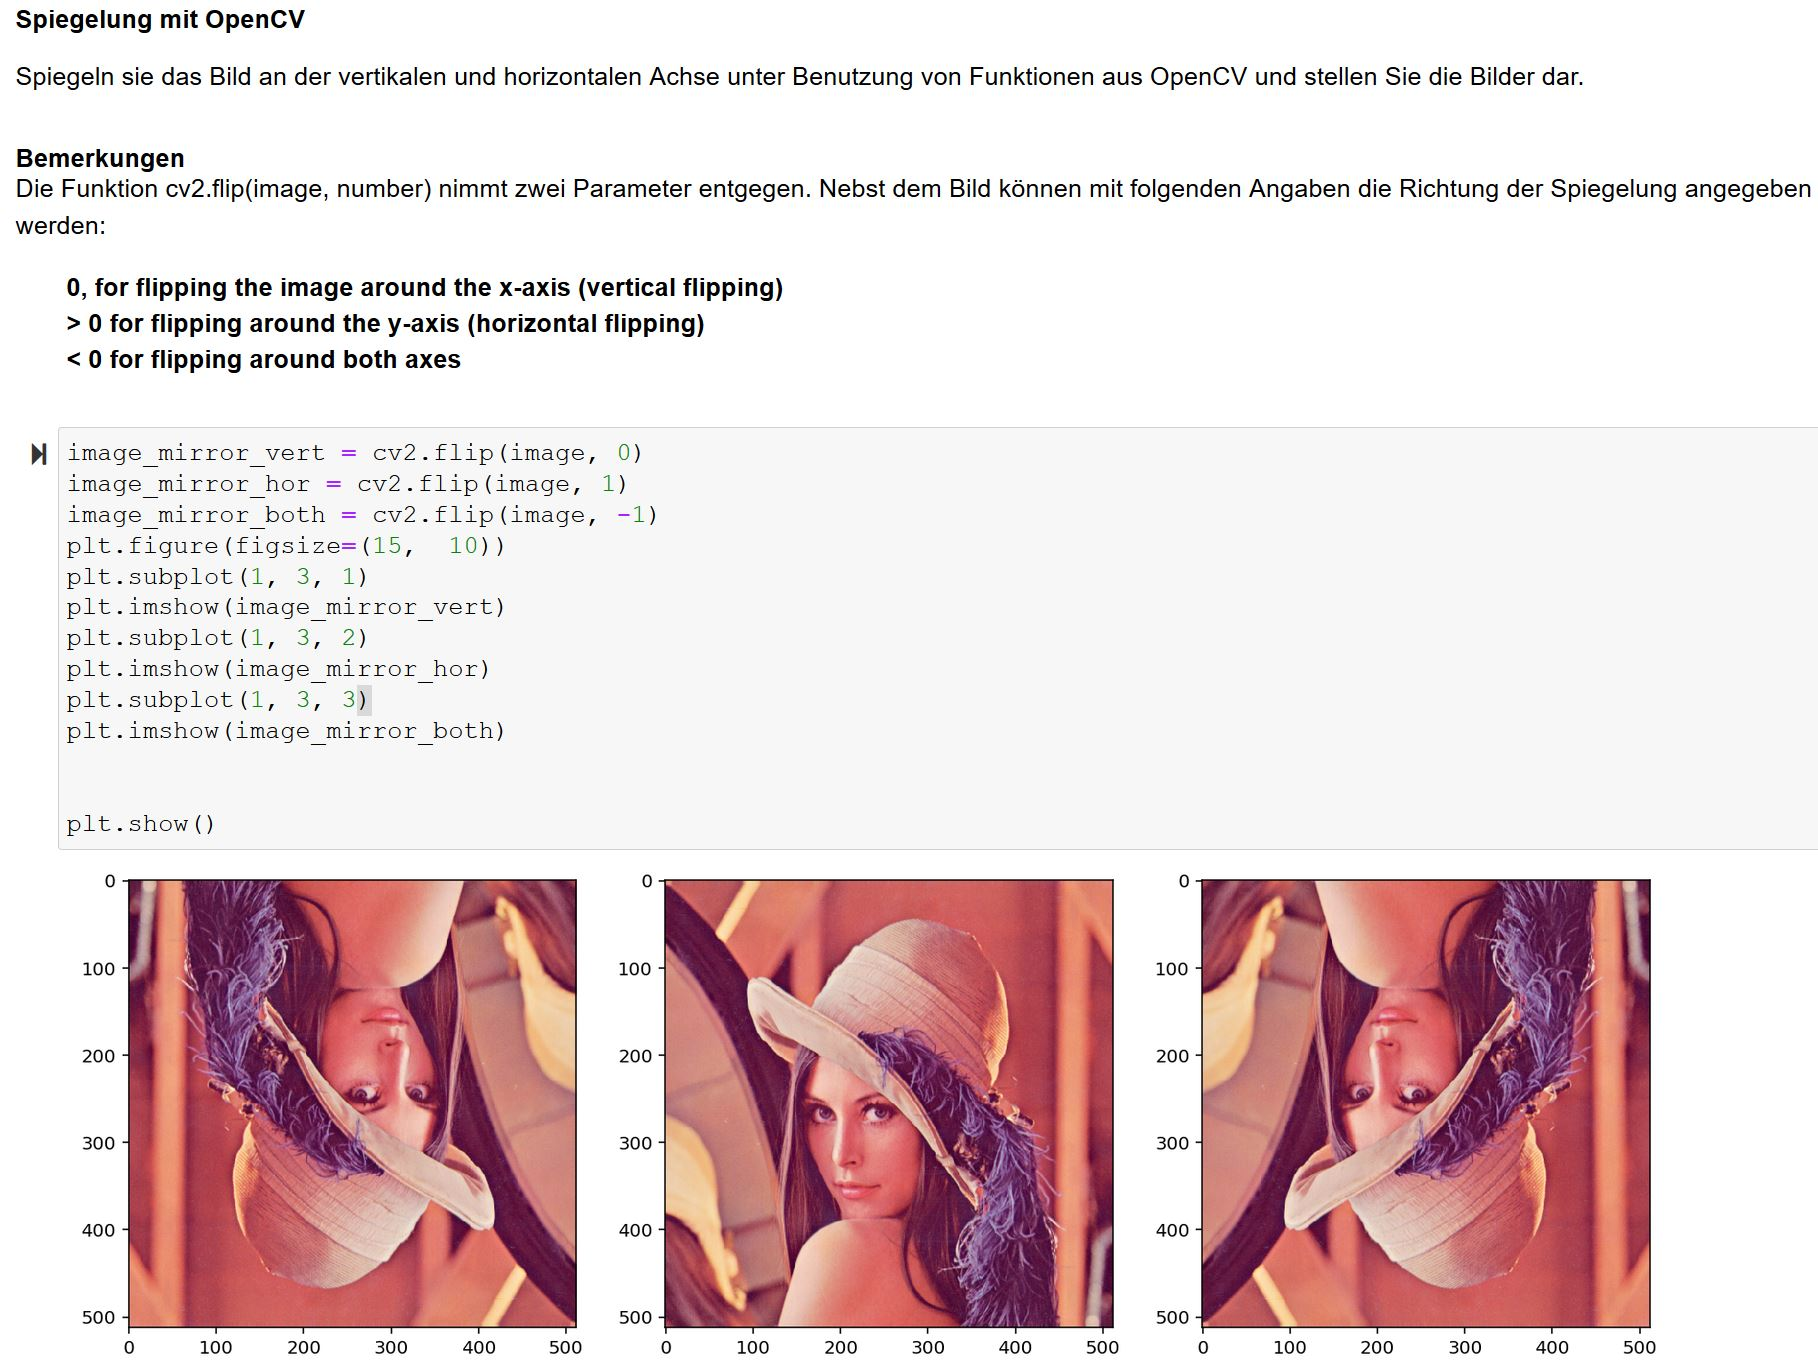
\includegraphics[height=10cm,keepaspectratio]{images/sw01/SpiegelungMitOpenCV.JPG}
\end{center}
\noindent
\textbf{Alternative Darstellung mit numpy} \newline
plt.subplot(1,2,1) \newline
plt.imshow(np.flip(image, 0)) \newline
plt.subplot(1,2,2) \newline
plt.imshow(np.flip(image,1)) \newline
plt.show()

\subsubsection{Kugeln zählen} 
\begin{center}
	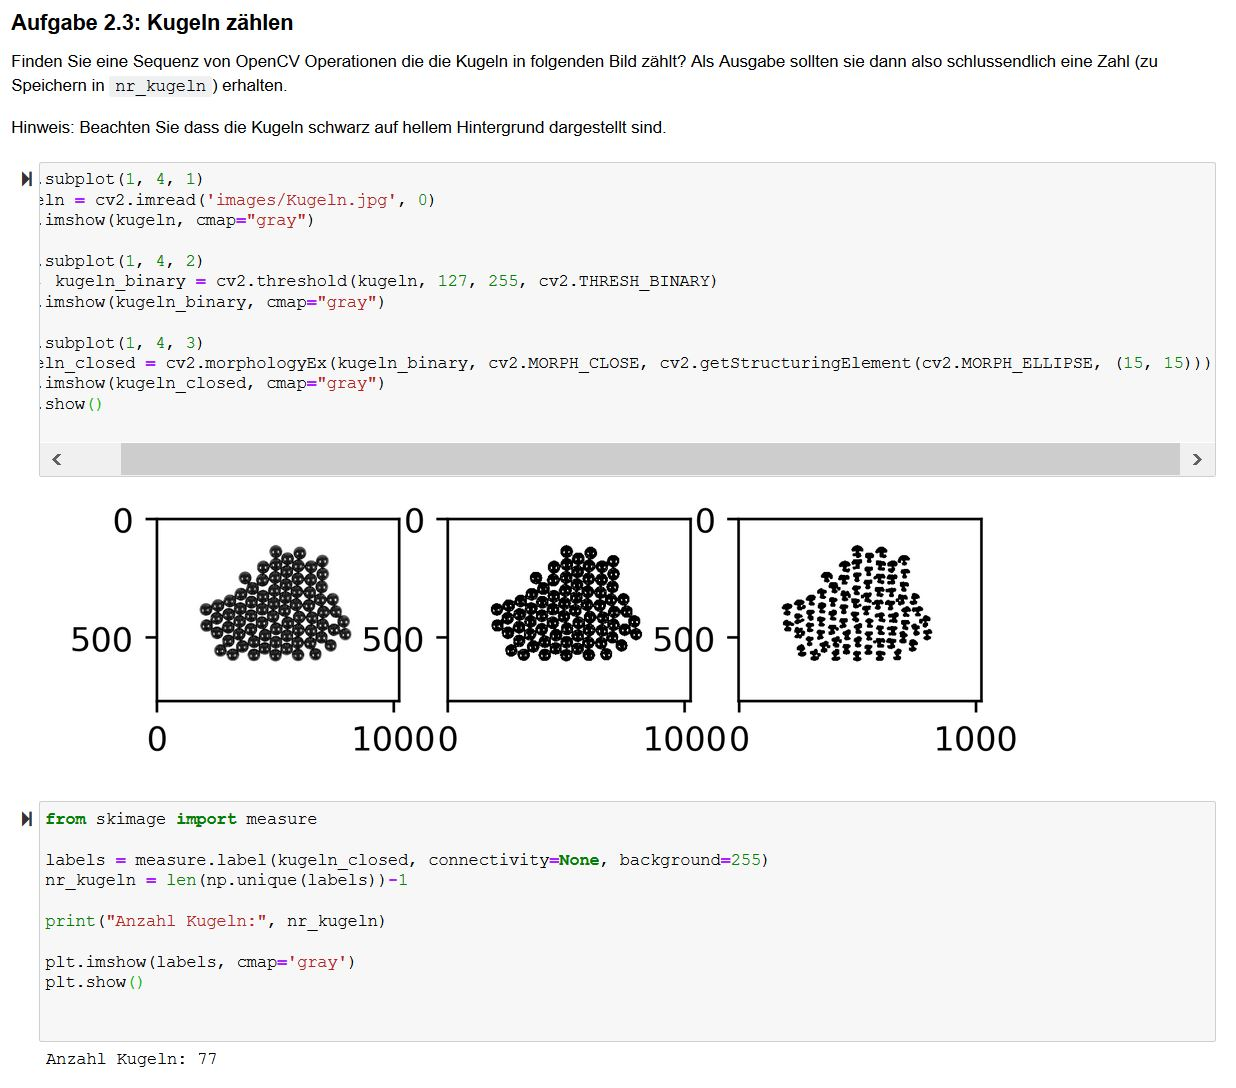
\includegraphics[height=13cm,keepaspectratio]{images/sw01/KugelnZaehlen.JPG}
\end{center}
Btw. die Lösung 77 ist korrekt








